\section{Introduction}

\subsection{Personal introduction}
\begin{itemize}
    \item Ich + paper + yad
\end{itemize}

\subsection{Goals and non-goals}
Let us quickly review the goals and also the non-goals:

Goals:
\begin{itemize}
    \item Make a meaningful comparison between the theoretical predictions and the experimental measurement of a fully inclusive DIS cross-section.
    \item Review pQCD features and exemplify them using DIS
\end{itemize}

Non-goals:
\begin{itemize}
    \item We only consider pQCD in the collinear framework here.
        However, because DIS is such a powerful experiment, which offers a clean access to the inner structure of the protons it can be studied using other frameworks as well, such as Color Glass Condensates~\cite{Bertilsson:2026vtu,Casuga:2026xxt} \textrightarrow{} ask H.~Mäntysaari or T.~Lappi
    \item We only consider fully inclusive cross-sections here (to be defined in \cref{sec:xs} and with a tiny exception to be discussed in \cref{sec:hq}).
        In particular, we will not consider any more complicated final states, such as, e.g.\ single jet or di-jet production~\cite{H1:2014cbm}.
    \item We only consider pQCD in the collinear framework here.
        While, Monte Carlo Event generators, such as, e.g. Pythia~\cite{Bierlich:2022pfr}, are rooted in collinear pQCD they eventually go much beyond and we do not consider their details here~\cite{Helenius:2026odp} \textrightarrow{} ask I.~Helenius.
\end{itemize}

\subsection{Requirements}

We need some basic knowledge from particle physics and, in particular, you need to be familiar with the Standard Model overview shown in \cref{fig:SM}.
\begin{figure}
    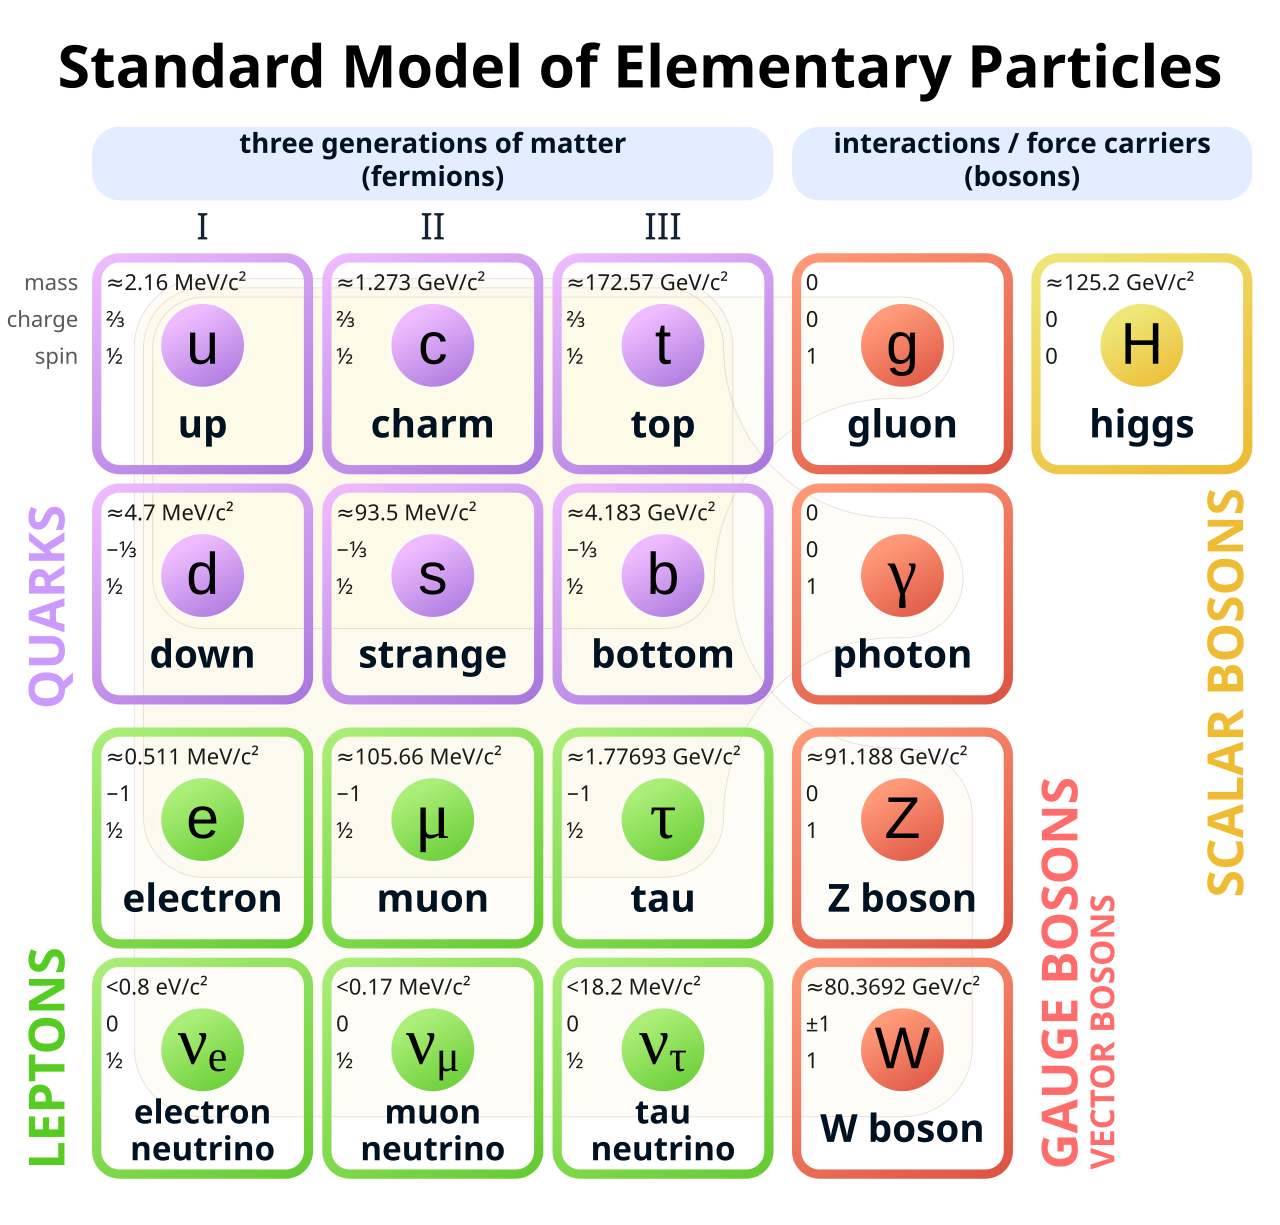
\includegraphics[width=.8\textwidth]{figures/Standard_Model_of_Elementary_Particles.svg.png}
    \caption{The Standard Model of Elementary Particles - taken from \cite{wikiSM}}
    \label{fig:SM}
\end{figure}
We will discuss in this course each and everyone of these particles, with the exception of the three heaviest in each category:
the heavies quark, the top, the heaviest lepton, the tau, and the heaviest boson, the Higgs.
They will work, in principle mostly like their lighter brothers and sisters, but in practice are basically always neglected.
We give a more thorough justification to discard them when we get to the actual numbers.
All other particles will explicitly appear in this course and you need to know their charges - see also \cref{fig:SM}.

\begin{tcolorbox}[title={Summary forces, particles, and charges}]
    \begin{itemize}
        \item The carrier of the strong force is the gluon
        \item Quarks have a strong charge, leptons don't
        \item The carriers of the electro-weak force are the photon, the Z boson, and the W boson
        \item Quarks and leptons have both electro-magnetic and weak charges
    \end{itemize}
\end{tcolorbox}

We also need some basic knowledge from Quantum Field Theory.

\subsection{The very basics}
\begin{itemize}
    \item D I S
    \item factorization theorem
    \item LO (+ NLOq + NLOg)
    \item IC
\end{itemize}
